
%(BEGIN_QUESTION)
% Copyright 2010, Tony R. Kuphaldt, released under the Creative Commons Attribution License (v 1.0)
% This means you may do almost anything with this work of mine, so long as you give me proper credit

This gas pressure control system has a problem.  The operator tells you that the pressure in the accumulator vessel pressure registers below setpoint on the pressure controller's display, and refuses to come up to setpoint.  He calls you to diagnose the problem in this system:

$$\includegraphics[width=15.5cm]{i01820x01.eps}$$

Your first diagnostic check is to note the percentage output signal on the pressure controller (PIC): the controller's display shows an output of 68\%.  Identify the likelihood of each possible cause in this list by checking boxes in the table -- whether the cause is ``probable'' (worth considering as a cause of this system's trouble) or is ``unlikely'' (either completely ruled out as a cause, or just not worth considering at this point in the diagnosis):

% No blank lines allowed between lines of an \halign structure!
% I use comments (%) instead, so that TeX doesn't choke.

$$\vbox{\offinterlineskip
\halign{\strut
\vrule \quad\hfil # \ \hfil & 
\vrule \quad\hfil # \ \hfil & 
\vrule \quad\hfil # \ \hfil \vrule \cr
\noalign{\hrule}
%
% First row
{\bf Fault} & {\bf Probable} & {\bf Unlikely} \cr
%
\noalign{\hrule}
%
% Another row
Control valve leaking (non-tight shutoff) &  & \cr
%
\noalign{\hrule}
%
% Another row
PT miscalibrated (reads too low) &  & \cr
%
\noalign{\hrule}
%
% Another row
PT miscalibrated (reads too high) &  & \cr
%
\noalign{\hrule}
%
% Another row
FT miscalibrated (reads too low) &  & \cr
%
\noalign{\hrule}
%
% Another row
FT miscalibrated (reads too high) &  & \cr
%
\noalign{\hrule}
%
% Another row
4-20 mA wiring to valve failed open &  & \cr
%
\noalign{\hrule}
%
% Another row
4-20 mA wiring to valve failed shorted &  & \cr
%
\noalign{\hrule}
%
% Another row
Excessive gas supply pressure &  & \cr
%
\noalign{\hrule}
%
% Another row
No integral action in pressure controller &  &  \cr
%
\noalign{\hrule}
} % End of \halign 
}$$ % End of \vbox


\vfil 

\underbar{file i01820}
\eject
%(END_QUESTION)





%(BEGIN_ANSWER)

This is a graded question -- no answers or hints given!

%(END_ANSWER)





%(BEGIN_NOTES)

% No blank lines allowed between lines of an \halign structure!
% I use comments (%) instead, so that TeX doesn't choke.

$$\vbox{\offinterlineskip
\halign{\strut
\vrule \quad\hfil # \ \hfil & 
\vrule \quad\hfil # \ \hfil & 
\vrule \quad\hfil # \ \hfil \vrule \cr
\noalign{\hrule}
%
% First row
{\bf Fault} & {\bf Probable} & {\bf Unlikely} \cr
%
\noalign{\hrule}
%
% Another row
Control valve leaking (non-tight shutoff) &  & $\surd$ \cr
%
\noalign{\hrule}
%
% Another row
PT miscalibrated (reads too low) &  & $\surd$ \cr
%
\noalign{\hrule}
%
% Another row
PT miscalibrated (reads too high) &  & $\surd$ \cr
%
\noalign{\hrule}
%
% Another row
FT miscalibrated (reads too low) &  & $\surd$ \cr
%
\noalign{\hrule}
%
% Another row
FT miscalibrated (reads too high) &  & $\surd$ \cr
%
\noalign{\hrule}
%
% Another row
4-20 mA wiring to valve failed open &  & $\surd$ \cr
%
\noalign{\hrule}
%
% Another row
4-20 mA wiring to valve failed shorted &  & $\surd$ \cr
%
\noalign{\hrule}
%
% Another row
Excessive gas supply pressure &  & $\surd$ \cr
%
\noalign{\hrule}
%
% Another row
No integral action in pressure controller & $\surd$ & \cr
%
\noalign{\hrule}
} % End of \halign 
}$$ % End of \vbox

One way to approach a problem like this is to put yourself in the position of the pressure controller: {\it what would you do if it was your task to manually control pressure inside this vessel?}  I'm willing to wager you would {\it not} leave the output signal at only 68\% if it was your goal to eliminate the error between the PV (too-low pressure) and the SP.

\vskip 10pt

If the controller's output were indeed saturated at or near 100\%, we might suspect a field instrument problem as the fault.  However, it is clear the PIC is not doing all it can to get the pressure up to setpoint, and so there is where we should focus our attention.

\vskip 10pt

A common misconception is to think that the FT is miscalibrated too high, causing the flow controller to regulate flow into the vessel at too low of a rate, thus causing the pressure to droop.  While this would indeed cause the actual flow rate to be less than setpoint, the pressure controller would simply call for more flow in order to reach its proper pressure setpoint.  Thus, a miscalibrated flow transmitter could not in and of itself cause pressure to be too low.  If the miscalibration were so severe that even at 100\% flow setpoint there still wasn't enough flow going into the vessel to raise its pressure to setpoint, we would see the pressure controller's output signal saturated at 100\% (not 68\% as the scenario describes).  This is how we know for sure the problem isn't an FT calibration issue.

Another misconception is that perhaps the PT is miscalibrated (too high), causing the pressure controller to regulate process pressure below the actual setpoint.  While such a miscalibration would indeed cause the actual process pressure to deviate from setpoint, it would {\it not} be evident from an inspection of the controller's display as we have been informed for this scenario.  The fact that the error may be seen from the controller's faceplate tells us the problem must lie elsewhere.

%INDEX% Basics, control loop troubleshooting: determining cause of process problem
%INDEX% Process: fuel gas receiver pressure control

%(END_NOTES)


